\documentclass[review]{elsarticle}

\usepackage{lineno,hyperref}
\usepackage{amsfonts,bm,amssymb,color,balance,graphicx,bm}
\usepackage{amsmath,amsthm}

\def \blkdiag{\operatorname{blkdiag}}
\def \diag{\operatorname{diag}}
\def \ln{\operatorname{ln}}
\def \arg{\operatorname{arg}}
\def \tr{\operatorname{tr}}
\modulolinenumbers[5]

\journal{Journal of \LaTeX\ Templates}

%%%%%%%%%%%%%%%%%%%%%%%
%% Elsevier bibliography styles
%%%%%%%%%%%%%%%%%%%%%%%
%% To change the style, put a % in front of the second line of the current style and
%% remove the % from the second line of the style you would like to use.
%%%%%%%%%%%%%%%%%%%%%%%

%% Numbered
%\bibliographystyle{model1-num-names}

%% Numbered without titles
%\bibliographystyle{model1a-num-names}

%% Harvard
%\bibliographystyle{model2-names.bst}\biboptions{authoryear}

%% Vancouver numbered
%\usepackage{numcompress}\bibliographystyle{model3-num-names}

%% Vancouver name/year
%\usepackage{numcompress}\bibliographystyle{model4-names}\biboptions{authoryear}

%% APA style
%\bibliographystyle{model5-names}\biboptions{authoryear}

%% AMA style
%\usepackage{numcompress}\bibliographystyle{model6-num-names}

%% `Elsevier LaTeX' style
\bibliographystyle{elsarticle-num}
%%%%%%%%%%%%%%%%%%%%%%%

\begin{document}

\begin{frontmatter}

\title{Elsevier \LaTeX\ template\tnoteref{mytitlenote}}
\tnotetext[mytitlenote]{Fully documented templates are available in the elsarticle package on \href{http://www.ctan.org/tex-archive/macros/latex/contrib/elsarticle}{CTAN}.}

%% Group authors per affiliation:
\author{Elsevier\fnref{myfootnote}}
\address{Radarweg 29, Amsterdam}
\fntext[myfootnote]{Since 1880.}

%% or include affiliations in footnotes:
\author[mymainaddress,mysecondaryaddress]{Elsevier Inc}
\ead[url]{www.elsevier.com}

\author[mysecondaryaddress]{Global Customer Service\corref{mycorrespondingauthor}}
\cortext[mycorrespondingauthor]{Corresponding author}
\ead{support@elsevier.com}

\address[mymainaddress]{1600 John F Kennedy Boulevard, Philadelphia}
\address[mysecondaryaddress]{360 Park Avenue South, New York}

\begin{abstract}

\end{abstract}

\begin{keyword}

\end{keyword}

\end{frontmatter}

\linenumbers

\section{Problem Formulation}
Given $Q$ adjacent narrow-band emitters and $L$ space separated base-stations which intercept the transmitted signals. Every base-station is equipped with an antenna array consisting of $M$ elements.To avoid the angle ambiguity, the carrier frequency is small than the inverse of the propagation time over the array aperture. Denote the $q$th emitter’s position by the vector of coordinates $\boldsymbol{p}_q\in \mathbb{R}^{D\times 1}$ (In general, $D=2$ for plane geometry or $D=3$ for solid geometry). The complex envelopes of the signals observed by the $j$th base-
station array are given by
\begin{align}\label{yjt}
\boldsymbol{y}_j(t)=\sum_{q=1}^Q\alpha_{q,j}\boldsymbol{a}_j(\boldsymbol{p}_q)s_q(t-\tau_j(\boldsymbol{p}_q)-\mathring{t}_q)+\boldsymbol{w}_{j}(t),\quad 0\leq t\leq T
\end{align}
where $\boldsymbol{y}_j(t)$ is the $j$th received signal, $\alpha_q,j$ is an unknown complex scalar representing the channel attenuation between the $q$th emitter and the $j$th base-station, $\boldsymbol{a}_j(\boldsymbol{p}_q)$ is the $j$th array response to the signal transmitted from position $\boldsymbol{p}_q$, and $s_q(t-\tau_j(\boldsymbol{p}_q)-\mathring{t}_q)$ is the copy of the $q$th transmitted signal waveform, which is transmitted at time $\mathring{t}_q$ and is received by the $j$th base-station after being delayed by $\tau_j(\boldsymbol{p}_q)$. The vector $\boldsymbol{w}_j(t)$ represents noise and interference observed by the $j$th array. The received signal can be partitioned into $L$ sections and the length of each section satisfies $T/L\gg \max{\tau_j(\boldsymbol{p}_q)}$ to avoid the delay ambiguity. The emitters are assumed to be stationary during the total observation time $T$. Each section can be Fourier transformed and the result of this process is given by the following equation:
\begin{align}\label{yjnl}
    \boldsymbol{y}_j(n,l)&=\sum_{q=1}^Q\alpha_{q,j}\boldsymbol{a}_j(\boldsymbol{p}_q)e^{-j2\pi f_n(\tau_j(\boldsymbol{p}_q)+\mathring{t}_q)}s_q(n,l)+\boldsymbol{w}_j(n,l)\\ \nonumber
    j&=1,...,N_r;n=1,...,N;l=1,...,L
\end{align}
where $\boldsymbol{y}_j(n,l)$ is the Fourier coefficient of the $l$th section of the $j$th received signal corresponding to frequency $f_n$, $s_q(n,l)$ is the $n$th Fourier coefficient of the $l$th section of the $q$th transmitted signal waveform, and $\boldsymbol{w}_j(n,l)$ represents the $n$th Fourier coefficient of the $l$th section of the noise waveform.

For compact representation, we define the following vectors:
\begin{align}\label{gamma}
    \boldsymbol{\gamma}_{j,q,n,l}(\boldsymbol{p}_q,\mathring{t}_q\vert s_q(n,l))\triangleq\boldsymbol{a}_j(\boldsymbol{p}_q)e^{-j2\pi f_n(\tau_j(\boldsymbol{p}_q)+\mathring{t}_q)}s_q(n,l)
\end{align}
Here we assume that the spectrum of transmitted signals, like the synchronization and training sequences in cellular systems, are known to location system but the transmitted time $\mathring{t}_q$ is unknown (which is assumed known in \cite{DPD2005}). We observe that all information about the emitter’s position is embedded in the vector $\boldsymbol{\gamma}_{j,q,n,l}$. This leads to the following representation of \eqref{yjnl}:
\begin{align}\label{yjnl2}
    \boldsymbol{y}_j(n,l)=\sum_{q=1}^Q\alpha_{q,j}\boldsymbol{\gamma}_{j,q,n,l}+\boldsymbol{w}_j(n,l)
\end{align}
In matrix notation, \eqref{yjnl2} becomes
\begin{align}
    \boldsymbol{y}_j(n,l)=\boldsymbol{\Gamma}_{j,n,l}(\boldsymbol{P},\mathring{\boldsymbol{t}})\boldsymbol{\alpha}_j+\boldsymbol{w}_j(n,l)
\end{align}
where  
\begin{align}\label{Gammajnl}
    \boldsymbol{\Gamma}_{j,n,l}(\boldsymbol{P},\mathring{\boldsymbol{t}})&\triangleq[\boldsymbol{\gamma}_{j,q,n,l},...,\boldsymbol{\gamma}_{j,q,n,l}]\in \mathbb{C}^{M\times Q}\\ \nonumber
    \boldsymbol{\alpha}_j&\triangleq[\alpha_{1,j},...,\alpha_{Q,j}]^T\in \mathbb{C}^{Q\times 1} 
\end{align}
$\boldsymbol{P},\mathring{\boldsymbol{t}}$ are the sets of emitters' positions and transmitted times respectively.
Collecting and catenating all the $N$ coefficients of the $l$th section of the $j$th received signal,
\begin{align}
    \boldsymbol{y}_j(l)=\boldsymbol{\Gamma}_{j,l}(\boldsymbol{P},\mathring{\boldsymbol{t}})\boldsymbol{\alpha}_j+\boldsymbol{w}_j(l)
\end{align}
where
\begin{align}\label{Gammajl}
    \boldsymbol{y}_j(l)&\triangleq[\boldsymbol{y}_j^T(1,l),...,\boldsymbol{y}_j^T(N,l)]^T\in \mathbb{C}^{NM\times 1}\\ \nonumber
    \boldsymbol{\Gamma}_{j,l}(\boldsymbol{P},\mathring{\boldsymbol{t}})&\triangleq[\boldsymbol{\Gamma}_{j,1,l}^T(\boldsymbol{P},\mathring{\boldsymbol{t}}),...,\boldsymbol{\Gamma}_{j,N,l}^T(\boldsymbol{P},\mathring{\boldsymbol{t}})]^T\in \mathbb{C}^{NM\times Q}\\ 
    \boldsymbol{w}_j(l)&\triangleq[\boldsymbol{w}_j^T(1,l),...,\boldsymbol{w}_j^T(N,l)]^T\in \mathbb{C}^{NM\times 1}\nonumber
\end{align}
The problem that we address now is stated as follow: Given the measurements $\lbrace\boldsymbol{y}_j(l)\rbrace_{j,l=1}^{N_r,L}$, how to efficiently and accurately estimate the locations of the emitters $\boldsymbol{P}$.

\section{the Concentrated Likelihood Function}
In this subsection, we will derive the \emph{Concentrated} Likelihood Function (CLF) that depends on the parameters of interest $\boldsymbol{P}$ and the auxiliary parameters $\mathring{\boldsymbol{t}}$. The transmitted times are conducive to acquiring the location information from the propagation delay $\tau_j(\boldsymbol{p})$ since the transmitted times are the same among base-stations. In fact, since $\boldsymbol{w}_j(l)$ are independent among different sections of different received signals and $\boldsymbol{w}_j(l)\sim N(\boldsymbol{0},\sigma^2\boldsymbol{I}_{NM})$, it can be shown that the Log Likelihood Function (LLF) after dropping the constant terms is given by,
\begin{align}
\mathcal{L}(\boldsymbol{P},\mathring{\boldsymbol{t}},\boldsymbol{\alpha})\triangleq-\sum_{j=1}^{N_r}\sum_{l=1}^L\Vert \boldsymbol{y}_j(l)-\boldsymbol{\Gamma}_{j,l}(\boldsymbol{P},\mathring{\boldsymbol{t}})\boldsymbol{\alpha}_j\Vert^2
\end{align}
where $\boldsymbol{P},\mathring{\boldsymbol{t}},\boldsymbol{\alpha}$ stand for any candidate values. Now, define the matrix
\begin{align}\label{Gammaj}
    \boldsymbol{\Gamma}_{j}(\boldsymbol{P},\mathring{\boldsymbol{t}})\triangleq[\boldsymbol{\Gamma}_{j,1}^T,...,\boldsymbol{\Gamma}_{j,L}^T]^T\in \mathbb{C}^{LNM\times Q}
\end{align}
it can be shown that \eqref{L} is equivalent to 
\begin{align}\label{L}
    \mathcal{L}(\boldsymbol{P},\mathring{\boldsymbol{t}},\boldsymbol{\alpha})=-\sum_{j=1}^{N_r}\Vert \boldsymbol{y}_j-\boldsymbol{\Gamma}_{j}(\boldsymbol{P},\mathring{\boldsymbol{t}})\boldsymbol{\alpha}_j\Vert^2
\end{align}
where $\boldsymbol{y}_j\triangleq[\boldsymbol{y}_j^T(1),...,\boldsymbol{y}_j^T(L)]^T$.Maximizing \eqref{L} jointly with respect to all parameters is extremely challenging. Yet, significant computational savings follow from the observation that for any given $\boldsymbol{P},\mathring{\boldsymbol{t}}$, the problem of finding the optimal $\lbrace \boldsymbol{\alpha}_j\rbrace _{j=1}^{N_r}$ becomes a linear least squares (LS) problem \cite{Golub1973The} whose solution is given by
\begin{align}
    \hat{\boldsymbol{\alpha}}_j=\boldsymbol{\Gamma}_{j}^\dagger(\boldsymbol{P},\mathring{\boldsymbol{t}})\boldsymbol{y}_j
\end{align}
where $\boldsymbol{\Gamma}_{j}^\dagger$ is the Moore-Penrose pseudo-inverse of $\boldsymbol{\Gamma}_{j}$ given by $(\boldsymbol{\Gamma}_{j}^H\boldsymbol{\Gamma}_{j})^{-1}\boldsymbol{\Gamma}_{j}^H$. Note here that $\boldsymbol{\Gamma}_{j}$ has full column rank and, therefore, $(\boldsymbol{\Gamma}_{j}^H\boldsymbol{\Gamma}_{j})^{-1}$ always exists. Now, by substituting $\lbrace \hat{\boldsymbol{\alpha}}_j\rbrace _{j=1}^{N_r}$ for $\boldsymbol{\alpha}$ back in \eqref{L} and resorting to some straightforward algebraic manipulations, we obtain the so-called \emph{concentrated} likelihood function,
\begin{align}\label{CLF}
    \mathcal{L}_c(\boldsymbol{P},\mathring{\boldsymbol{t}})=\sum_{j=1}^{N_r}\boldsymbol{y}_j^H\boldsymbol{\Gamma}_{j}(\boldsymbol{\Gamma}_{j}^H\boldsymbol{\Gamma}_{j})^{-1}\boldsymbol{\Gamma}_{j}^H\boldsymbol{y}_j
\end{align}
The joint Maximum Likelihood (ML) estimates of $\boldsymbol{P}$ and $\mathring{\boldsymbol{t}}$ are then obtained as the solution to the following reduced-dimension optimization problem
\begin{align}\label{MLE}
    [\hat{\boldsymbol{P}},\hat{\mathring{\boldsymbol{t}}}]=arg \max_{\boldsymbol{P},\mathring{\boldsymbol{t}}} \mathcal{L}_c(\boldsymbol{P},\mathring{\boldsymbol{t}})
\end{align}
The reduced-dimension optimization problem \eqref{MLE} still has $Q(D+1)$ unknown parameters (including the $D$-dimensional real-valued location vectors $\lbrace \boldsymbol{p}_q\rbrace_{q=1}^Q$ and $Q$ transmitted times $\lbrace \mathring{t}_q\rbrace_{q=1}^Q$) remain to estimate. The ML estimation will therefore requires a complex multidimensional search over the parameter space.

To solve the multidimensional optimization problem \eqref{MLE}, the approach proposed in \cite{DPD2005} is to decouple the problem into several $D$-dimensional optimization problems under the assumption that the number of sections $L\to \infty$ or $L$ is sufficiently large in practice. Considering the length of section has low limit $T/L\gg \max{\tau_j(\boldsymbol{p}_q)}$, the number of sections $L$ is proportional to the total observation time $T$. The observation time $T$ is, however, limited in some practical reasons, like the request for real-time processing or the assumption that emitters are stationary during the observation. It is, therefore, difficult to be satisfied that $L$ is sufficiently large in some practical cases, which means the decouple approach proposed in \cite{DPD2005} may be failure, especially when the emitters are adjacent to one another.

\section{Global Maximization of The CLF}
As done previously within other estimation problems (see \cite{ISdoa2008,Kay2000Mean,Saha2002Maximum,Wang2010Maximum,Chen2008Joint}), we resort to the optimization framework, which is based on the Pincus' theorem and the powerful Importance Sampling (IS) method, to efficiently and accurately estimate the adjacent emitters' positions using limited observation time.
First of all, we introduce the theorem of Pincus \cite{Pincus1968A} as follows.
\theoremstyle{definition} \newtheorem{Theorem}{Theorem}
\begin{Theorem}
    Let $F(x_1,...,x_n)=F(\boldsymbol{x})$ be a continuous function on the closure of a bounded domain $S$ in $n$-dimensional Euclidean space of $\mathbb{R}^n$. Assume that $F$ attains a global maximum at exactly on point $\hat{\boldsymbol{x}}=[\hat{x}_1,...,\hat{x}_n]^T$ of $S$. Then for $i=1,...,n$,
    \begin{align}\label{Pincus}
    \hat{x}_i=\lim_{\rho\to \infty}\frac{\idotsint x_i e^{\rho F(\boldsymbol{x})}dx_1\cdots dx_n}{\idotsint e^{\rho F(\boldsymbol{x})}dx_1\cdots dx_n}
    \end{align}
\end{Theorem}
Applying this general result to our multidimensional optimization problem \eqref{MLE} with $\boldsymbol{x}\triangleq[\boldsymbol{P},\mathring{\boldsymbol{t}}]$ and $F(\boldsymbol{x})\triangleq \mathcal{L}_c(\boldsymbol{P},\mathring{\boldsymbol{t}})$ leads to the following expressions for the required ML estimators,
\begin{align}\label{MI1}
    \hat{\boldsymbol{p}}_q(d)=\idotsint \boldsymbol{p}_q(d) \mathcal{F}(\boldsymbol{P},\mathring{\boldsymbol{t}})d\boldsymbol{p}_1(1) \cdots d\mathring{t}_Q
\end{align}
\begin{align}\label{MI2}    
    \hat{t}_q^{(0)}&=\idotsint \mathring{t}_q \mathcal{F}(\boldsymbol{P},\mathring{\boldsymbol{t}})d\boldsymbol{p}_1(1) \cdots d\mathring{t}_Q\\ 
    q&=1,...,Q;d=1,...,D \nonumber
\end{align}
where 
\begin{align}\label{gc}
    \mathcal{F}(\boldsymbol{P},\mathring{\boldsymbol{t}})\triangleq\lim_{\rho\to \infty}\frac{e^{\rho \mathcal{L}_c(\boldsymbol{P},\mathring{\boldsymbol{t}})}}{\idotsint e^{\rho \mathcal{L}_c(\boldsymbol{P},\mathring{\boldsymbol{t}})}d\boldsymbol{p}_1(1) \cdots d\mathring{t}_Q}
\end{align}
Intuitively, as $\rho$ tends to infinity, $\mathcal{F}(\boldsymbol{P},\mathring{\boldsymbol{t}})$ becomes a Dirac-delta function centered at the maximum of $\mathcal{L}_c(\boldsymbol{P},\mathring{\boldsymbol{t}})$ whose location is indeed given by the set of integrals in \eqref{MI1} and \eqref{MI2}. It however, seems that the multidimensional grid search we attempt to avoid is transformed into several multidimensional integrations \eqref{MI1} and \eqref{MI2} bearing the same computational load. By closely analyzing the properties of function \eqref{gc}, fortunately, it turns out that $\mathcal{F}(\boldsymbol{P},\mathring{\boldsymbol{t}})$ can be seen as a Probability Density Function (pdf) since it is nonnegative and integrates to one. As a pdf, furthermore, $\mathcal{F}(\boldsymbol{P},\mathring{\boldsymbol{t}})$ indicates the probability of the candidate values being true. The estimators in \eqref{MI1} and \eqref{MI2} can be regarded as statistical expectations, i.e., we have,
\begin{align}\label{ex}
    \hat{\boldsymbol{p}}_q(d)\triangleq \mathbb{E}_{\boldsymbol{P},\mathring{\boldsymbol{t}}}\{\boldsymbol{p}_q(d)\} \quad \hat{\mathring{t}}_q\triangleq \mathbb{E}_{\boldsymbol{P},\mathring{\boldsymbol{t}}}\{\mathring{t}_q\}
\end{align}
Consequently, the multidimensional integrations are transformed into the statistical expectations, which can be approximated by the sample mean. 
We will then explain the method to generate $R$ realizations, $\lbrace \boldsymbol{P}^{(r)}\rbrace_{r=1}^R$ and $\lbrace \mathring{\boldsymbol{t}}^{(r)}\rbrace_{r=1}^R$, using the joint pdf $\mathcal{F}(\boldsymbol{P},\mathring{\boldsymbol{t}})$ and approximate the expectations in \eqref{ex} using the following sample means,
\begin{align}\label{SM}
    \hat{\boldsymbol{p}}_q(d)=\frac{1}{R}\sum_{r=1}^R \boldsymbol{p}_q^{(r)}(d) \quad \hat{\mathring{t}}_q=\frac{1}{R}\sum_{r=1}^R \mathring{t}_q^{(r)}
\end{align}
Clearly, as the number of realizations $R$ increases, the two sample mean in \eqref{SM} approach the statistical expectations in \eqref{ex}. Unfortunately, the extremely non-linear property of the pdf $\mathcal{F}(\boldsymbol{P},\mathring{\boldsymbol{t}})$ makes it impractical to generate $\lbrace \boldsymbol{P}^{(r)}\rbrace_{r=1}^R$ and $\lbrace \mathring{\boldsymbol{t}}^{(r)}\rbrace_{r=1}^R$ using itself. To sidestep this problem, we can resort to the Importance Sampling (IS) method \cite{ISdoa2008,Kay2000Mean} and rewrite \eqref{MI1} and \eqref{MI2} in the following equivalent forms,
\begin{align}\label{IS-P}
    \hat{\boldsymbol{p}}_q(d)=\idotsint \boldsymbol{p}_q(d) \frac{\mathcal{F}(\boldsymbol{P},\mathring{\boldsymbol{t}})}{\mathcal{G}(\boldsymbol{P},\mathring{\boldsymbol{t}})}\mathcal{G}(\boldsymbol{P},\mathring{\boldsymbol{t}})d\boldsymbol{p}_1(1) \cdots d\mathring{t}_Q
\end{align}
\begin{align}\label{IS-t}    
    \hat{\mathring{t}}_q&=\idotsint \mathring{t}_q \frac{\mathcal{F}(\boldsymbol{P},\mathring{\boldsymbol{t}})}{\mathcal{G}(\boldsymbol{P},\mathring{\boldsymbol{t}})}\mathcal{G}(\boldsymbol{P},\mathring{\boldsymbol{t}})d\boldsymbol{p}_1(1) \cdots d\mathring{t}_Q
\end{align}
where $\mathcal{G}(\boldsymbol{P},\mathring{\boldsymbol{t}})$ is another pdf called \emph{importance function} (IF). By introducing the IF, the multidimensional integrations in \eqref{IS-P} and \eqref{IS-t} are interpreted as statistical expectations of two transformed random variates (RVs), i.e.,
\begin{align}\label{IS-ex}
    \hat{\boldsymbol{p}}_q(d)\triangleq \mathbb{E}_{\boldsymbol{P},\mathring{\boldsymbol{t}}}\{\eta(\boldsymbol{P},\mathring{\boldsymbol{t}})\boldsymbol{p}_q(d)\} \quad \hat{\mathring{t}}_q\triangleq \mathbb{E}_{\boldsymbol{P},\mathring{\boldsymbol{t}}}\{\eta(\boldsymbol{P},\mathring{\boldsymbol{t}})\mathring{t}_q\}
\end{align}
where $\eta(\boldsymbol{P},\mathring{\boldsymbol{t}})$ is called \emph{importance weight} (IW) corresponding to the realizations of $\boldsymbol{P},\mathring{\boldsymbol{t}}$ and defined as,
\begin{align}\label{eta}
    \eta(\boldsymbol{P},\mathring{\boldsymbol{t}})\triangleq\frac{\mathcal{F}(\boldsymbol{P},\mathring{\boldsymbol{t}})}{\mathcal{G}(\boldsymbol{P},\mathring{\boldsymbol{t}})}
\end{align}
If $\mathcal{G}(\boldsymbol{P},\mathring{\boldsymbol{t}})$ is carefully designed, the expectations in \eqref{IS-ex} can be computed at any desired degree of accuracy (by increasing $R$) using the corresponding sample mean estimates. In fact, the choice of $\mathcal{G}(\boldsymbol{P},\mathring{\boldsymbol{t}})$ is a tradeoff between the ease and efficiency of sampling. The appropriate choice of the IF will be discussed in the following section. 

\section{Appropriate Choice of Importance Function}
The appropriate $\mathcal{G}(\boldsymbol{P},\mathring{\boldsymbol{t}})$ must be designed as close as possible to $\mathcal{F}(\boldsymbol{P},\mathring{\boldsymbol{t}})$ while allowing at the same time the easy generation of the required parameters realizations $\lbrace \boldsymbol{P}^{(r)}\rbrace_{r=1}^R$ and $\lbrace \mathring{\boldsymbol{t}}^{(r)}\rbrace_{r=1}^R$. 
In order to facilitate the process of generating the required $R$ parameter realizations, we constrain IF's form separable in terms of the $Q$ position-transmitted time pairs $\lbrace(\boldsymbol{p}_q,\mathring{t}_q)\rbrace_{q=1}^Q$. In other words, our ultimate goal is to design $\mathcal{G}(\boldsymbol{P},\mathring{\boldsymbol{t}})$ in a way that allows it to be factorized as follows,
\begin{align}\label{SForm}
    \mathcal{G}(\boldsymbol{P},\mathring{\boldsymbol{t}})\triangleq \prod_{q=1}^Q g_q(\boldsymbol{p}_q,\mathring{t}_q)
\end{align}
This allow us to interpret the pdf of $Q(D+1)$-dimensional random vector as the joint pdf of $Q$ independent $(D+1)$-dimensional random vectors. Hence, we can independently generate $Q$ groups of realizations for $(D+1)$-dimensional random vectors $\lbrace(\boldsymbol{p}_q^{(r)},\mathring{t}_q^{(r)})\rbrace_{r,q=1}^{R,Q}$, instead of generating realizations for $Q(D+1)$-dimensional random vector $(\boldsymbol{P},\mathring{\boldsymbol{t}})$ directly using $\mathcal{G}(\boldsymbol{P},\mathring{\boldsymbol{t}})$. 

We start with the CLF \eqref{CLF}, the separable form \eqref{SForm} requests that the CLF has summation form with respect to $q$. Note that the product $\boldsymbol{y}_j^H\boldsymbol{\Gamma}_{j}$ in CLF is a $Q$-dimensional vector. Diagonalizing the inverse matrix $(\boldsymbol{\Gamma}_{j}^H\boldsymbol{\Gamma}_{j})^{-1}$ is, therefore, the key step to the separable form \eqref{SForm}. According to the definition of $\boldsymbol{\Gamma}_{j}$ in \eqref{Gammaj},  $\boldsymbol{\Gamma}_{j,l}$ in \eqref{Gammajl}, $\boldsymbol{\Gamma}_{j,n,l}$ in \eqref{Gammajnl} and $\boldsymbol{\gamma}_{j,q,n,l}$ in \eqref{gamma}, the $(u,v)$th element of the matrix product $\boldsymbol{\Gamma}_{j}^H\boldsymbol{\Gamma}_{j}$ is given by,
\begin{align*}
    [\boldsymbol{\Gamma}_{j}^H\boldsymbol{\Gamma}_{j}]_{u,v}&=\sum_{l=1}^L\sum_{n=1}^N \boldsymbol{\gamma}_{j,q,n,l}^H\boldsymbol{\gamma}_{j,q,n,l}\\
    &=\underbrace{\boldsymbol{a}_j^H(\boldsymbol{p}_u)\boldsymbol{a}_j(\boldsymbol{p}_u)}_{r_{doa,j}^{(u,v)}}\underbrace{\sum_{n=1}^N e^{j2\pi f_n(\tau_j(\boldsymbol{p}_u)+\mathring{t}_u-\tau_j(\boldsymbol{p}_v)-\mathring{t}_v)}}_{r_{toa,j}^{(u,v)}}\underbrace{\sum_{l=1}^L s_u^\ast(n,l)s_v(n,l)}_{r_{s}^{(u,v)}}
\end{align*}
where $r_{doa,j}^{(u,v)}, r_{toa,j}^{(u,v)}, r_{s}^{(u,v)}$ denote the $(u,v)$th non-normalized correlation coefficients in aspects of Direction Of Arrival (DOA) and Time Of Arrival (TOA) at the $j$th base-station and the transmitted signal, respectively. The matrix $\boldsymbol{\Gamma}_{j}^H\boldsymbol{\Gamma}_{j}$ is, therefore, a correlation matrix among all emitters. To avoid additional computational load, we directly assume, instead of strict diagonalizing, $\boldsymbol{\Gamma}_{j}^H\boldsymbol{\Gamma}_{j}$, as diagonal matrix, at the cost of losing the correlation information. The diagonal matrix, for $j=1,...,N_r$, is given by,
\begin{align}\label{GammaDiag}
    \boldsymbol{\Gamma}_{j}^H\boldsymbol{\Gamma}_{j}=MNL\cdot \boldsymbol{I}
\end{align}
where $\boldsymbol{I}$ is the identity matrix, the coefficient $MNL$ is the diagonal element of $\boldsymbol{\Gamma}_{j}^H\boldsymbol{\Gamma}_{j}$. 

substituting \eqref{GammaDiag} into \eqref{CLF} and ignoring the constant coefficient, we get its separated form as follows,
\begin{align}\label{GLc}
    \tilde{\mathcal{L}}_c(\boldsymbol{P},\mathring{\boldsymbol{t}})&= \sum_{j=1}^{N_r}\Vert \boldsymbol{\Gamma}_{j}^H\boldsymbol{y}_j\Vert ^2\\
    &=\sum_{q=1}^Q \tilde{\ell}_c(\boldsymbol{p}_q,\mathring{t}_q)
\end{align}
where 
\begin{align}\label{glc}
    \tilde{\ell}_c(\boldsymbol{p}_q,\mathring{t}_q)\triangleq \sum_{j,n,l=1}^{N_r,N,L} \vert \boldsymbol{\gamma}_{j,q,n,l}^H\boldsymbol{y}_j(n,l)\vert ^2
\end{align}

Replacing $\mathcal{L}_c(\boldsymbol{P},\mathring{\boldsymbol{t}})$ and $\rho$ in \eqref{gc} with $\tilde{\mathcal{L}}_c(\boldsymbol{P},\mathring{\boldsymbol{t}})$ and an appropriate $\rho_2$, we get the separated form of $\mathcal{G}(\boldsymbol{P},\mathring{\boldsymbol{t}})$ \eqref{SForm} and the $q$th component is given by,
\begin{align}\label{gq}
    g_q(\boldsymbol{p}_q,\mathring{t}_q)\triangleq\frac{e^{\rho_2 \tilde{\ell}_c(\boldsymbol{p}_q,\mathring{t}_q)}}{\int\int e^{\rho_2 \tilde{\ell}_c(\boldsymbol{p}_q,\mathring{t}_q)}d\boldsymbol{p}_qd\mathring{t}_q }
\end{align}
The generation of $q$th group of realizations $\lbrace(\boldsymbol{p}_q^{(r)},\mathring{t}_q^{(r)})\rbrace_{r=1}^{R}$ follows, furthermore, the well-known general result from probability theory, which is that the joint pdf, $g_q(\boldsymbol{p}_q,\mathring{t}_q)$, can be factorized as the product of marginal and conditional pdfs,
\begin{align}
    g_q(\boldsymbol{p}_q,\mathring{t}_q)=g_{q}^{\text{mar}}(\boldsymbol{p}_q)g_{q}^{\text{con}}(\mathring{t}_q\vert \boldsymbol{p}_q)
\end{align}

The usual method to obtain the marginal pdf $g_{q}^{\text{mar}}(\boldsymbol{p}_q)$ is integrating the joint pdf $g_q(\boldsymbol{p}_q,\mathring{t}_q)$ with respect to the transmitted time $\mathring{t}_q$. The analytical  integration is, however, difficult since $g_q(\boldsymbol{p}_q,\mathring{t}_q)$ has very high non-linear about $\mathring{t}_q$. The discrete approximation is also involving $D+1$-dimensional grid search. We have another alternative method to construct $ g_{q}^{\text{mar}}(\boldsymbol{p}_q)$ directly and efficiently,
\begin{align}\label{gmar}
    g_{q}^{\text{mar}}(\boldsymbol{p}_q)\triangleq\frac{e^{\rho_1\ell(\boldsymbol{p}_q)}}{\int e^{\rho_1\ell(\boldsymbol{p}_q)} d\boldsymbol{p}_q}
\end{align} 
where $\ell(\boldsymbol{p}_q)$ is the \emph{single} ($Q=1$) Likelihood Function (SLF) of the position $\boldsymbol{p}_q$ , which is derived from \eqref{glc} by eliminating the transmitted time $\mathring{t}_q$. We will, then, describe the derivation in details. 

Our derivation starts with a vector definition as follows,
\begin{align}\label{gammaqjl}
    \boldsymbol{\gamma}_{q,j,l}\triangleq\boldsymbol{\Phi}_{q,j,l}(\boldsymbol{p}_q)\boldsymbol{b}(\mathring{t}_q)
\end{align}
where
\begin{align}\label{Phi}
    \boldsymbol{\Phi}_{q,j,l}(\boldsymbol{p}_q)&\triangleq\boldsymbol{\Lambda}_j(\boldsymbol{p}_q,s_q(l))\otimes \boldsymbol{a}_j(\boldsymbol{p}_q)\\
    \boldsymbol{b}(\mathring{t}_q)&\triangleq[e^{-j2\pi f_1\mathring{t}_q},...,e^{-j2\pi f_N\mathring{t}_q}]^T\\
    \boldsymbol{\Lambda}_j(\boldsymbol{p}_q,s_q(l))&\triangleq 
    \left[ 
    \begin{array}{ccc}
        s_q(1,l)e^{-j2\pi f_1\tau_j(\boldsymbol{p}_q)}& \ldots & 0\\
        \vdots&\ddots&\vdots\\
        0&\ldots&s_q(N,l)e^{-j2\pi f_N\tau_j(\boldsymbol{p}_q)}
    \end{array}
    \right ]   
\end{align}
substituting \eqref{gammaqjl} and \eqref{Phi} into \eqref{glc}, we get
\begin{align}
    \tilde{\ell}_c(\boldsymbol{p}_q,\mathring{t}_q)&= \sum_{j=1}^{N_r} \sum_{l=1}^{L} \boldsymbol{\gamma}_{j,q,l}^H\boldsymbol{y}_j(l)\boldsymbol{y}_j^H(l)\boldsymbol{\gamma}_{j,q,l}\\
    &=\boldsymbol{b}^H(\mathring{t}_q)\underbrace{\left(\sum_{j=1}^{N_r} \sum_{l=1}^{L} \boldsymbol{\Phi}^H_{q,j,l}(\boldsymbol{p}_q)\boldsymbol{y}_j(l)\boldsymbol{y}_j^H(l)\boldsymbol{\Phi}_{q,j,l}(\boldsymbol{p}_q)\right)}_{\triangleq\boldsymbol{\Pi}_q(\boldsymbol{p}_q)} \boldsymbol{b}(\mathring{t}_q)
\end{align}
The right hand of the second equation is a non-normalized Rayleigh Quotient with respect to $\mathring{t}_q$. Consequently, maximizing $\tilde{\ell}_c(\boldsymbol{p}_q,\mathring{t}_q)$ with respect to $\mathring{t}_q$, we get,
\begin{align}\label{ell_lambda}
    \ell_q(\boldsymbol{p}_q)\triangleq\lambda_{\text{max}}(\boldsymbol{\Pi}_q(\boldsymbol{p}_q))
\end{align}
Substituting \eqref{ell_lambda} into \eqref{gmar}, we get the marginal pdf of the $q$th emitter's position,
\begin{align}\label{gpq}
    g_{q}^{\text{mar}}(\boldsymbol{p}_q)=\frac{e^{\rho_1\lambda_{\text{max}}(\boldsymbol{\Pi}_q(\boldsymbol{p}_q))}}{\int e^{\rho_1\lambda_{\text{max}}(\boldsymbol{\Pi}_q(\boldsymbol{p}_q))} d\boldsymbol{p}_q}
\end{align}
Given position realization $\boldsymbol{p}_q^{(r)}$ generated by $g_{q}^{\text{mar}}(\boldsymbol{p}_q)$, the conditional transmitted time pdf is defined as,
\begin{align}\label{Conpdf}
    g_{q}^{\text{con}}(\mathring{t}_q\vert \boldsymbol{p}_q^{(r)})=\frac{g_q(\boldsymbol{p}_q^{(r)},\mathring{t}_q)}{\int_{\mathring{t}}g_q(\boldsymbol{p}_q^{(r)},\mathring{t}_q)d\mathring{t}}
\end{align}
Substituting \eqref{gq} into \eqref{Conpdf}, we have,
\begin{align}\label{gtq}
    g_{q}^{\text{con}}(\mathring{t}_q\vert \boldsymbol{p}_q^{(r)})=\frac{e^{\rho_2 \tilde{\ell}_c(\boldsymbol{p}^{(r)}_q,\mathring{t}_q)}}{\int_{\mathring{t}}e^{\rho_2 \tilde{\ell}_c(\boldsymbol{p}^{(r)}_q,\mathring{t}_q)}d\mathring{t}}
\end{align}
Note that we use $\int_{\mathring{t}}e^{\rho_2 \tilde{\ell}_c(\boldsymbol{p}^{(r)}_q,\mathring{t}_q)}d\mathring{t}$, instead of $g_{q}^{\text{mar}}(\boldsymbol{p}_q^{(r)})$, to normalize the conditional pdf \eqref{Conpdf} correctly. 

The process of generating the required realizations $\lbrace(\boldsymbol{p}_q^{(r)},\mathring{t}_q^{(r)})\rbrace_{r,q=1}^{R,Q}$ are as follows: for $q$th group of realizations, generate $\lbrace \boldsymbol{p}_q^{(r)}\rbrace_{r=1}^R$ using the marginal pdf $g_{q}^{\text{mar}}(\boldsymbol{p}_q)$ \eqref{gpq} and then use the conditional pdf $g_{q}^{\text{con}}(\mathring{t}_q\vert \boldsymbol{p}_q^{(r)})$ \eqref{gtq} to generate $\lbrace \mathring{t}_q\rbrace_{r=1}^R$.

\section{Generations Of The Required Realizations}
We recall the following lemma \cite{Kay2006Intuitive} that will be used to generate the required realizations:
\theoremstyle{definition} \newtheorem{Lemma}{Lemma}
\begin{Lemma}\label{Lemma1}
    Let $X \in \mathcal{X}$ be any RV with pdf $f_X(x)$ and the Cumulative Distribution Function (CDF) $F_X(x)$ and denote the inverse CDF as $F_X^{-1}(\cdot)$ : $[0,1]\to \mathcal{X},  u\to x \; s.t. F_X(x)=u$. Then, for any uniform RV, $U\in [0,1]$, the RV $\tilde{X}=F_X^{-1}(U)$ is distributed according to $f_X(\cdot)$.
\end{Lemma}
According to the generating process described before, firstly, we should use the marginal pdf $g_{q}^{\text{mar}}(\boldsymbol{p}_q)$ \eqref{gpq} to generate $\lbrace \boldsymbol{p}_q^{(r)}\rbrace_{r=1}^R$. $g_{q}^{\text{mar}}(\boldsymbol{p}_q)$ is, however, unsuitable to be used along with the result of Lemma \ref{Lemma1} since $\boldsymbol{p}_q$ is a $D$-dimensional vector (defining $\boldsymbol{p}_q=(x_q,y_q)$ for $D=2$) instead of a scalar. To acquire the $D=2$ scalar pdfs, consequently, $g_{q}^{\text{mar}}(\boldsymbol{p}_q)$ should be factorized as follows,
\begin{align}
    g_{q}^{\text{mar}}(x_q,y_q)\triangleq g_{x}^{\text{mar}}(x_q)g_{y\vert x}^{\text{con}}(y_q\vert x_q)
\end{align}
where 
\begin{align}\label{gxgy}
    g_{x}^{\text{mar}}(x_q)&\triangleq \int g_{q}^{\text{mar}}(x_q,y_q) dy_q\\
    g_{y\vert x}^{\text{con}}(y_q\vert x_q)&\triangleq \frac{g_{q}^{\text{mar}}(x_q,y_q)}{g_{x}^{\text{mar}}(x_q)}
\end{align}
In conclusion, the approach of generating the $q$th group of realizations $\lbrace(\boldsymbol{p}_q^{(r)},\mathring{t}_q^{(r)})\rbrace_{r=1}^{R}$ can be stated as follows: generate $R$ realizations $\lbrace u_x^{(r)}\rbrace_{r=1}^R\sim U[0,1]$ and obtain $x_q^{(r)}=G_{x_q}^{-1}(u_x^{(r)})$ where $G_{x_q}(\cdot)$ is the CDF associated to $g_{x}^{\text{mar}}(x_q)$ in \eqref{gxgy}; For $r=1,...,R$, then, generate two realizations $u_y^{(r)},u_{\mathring{t}}^{(r)}\sim U[0,1]$ and obtain $y_q^{(r)}=G_{y_q\vert x_q^{(r)}}^{-1}(u_y^{(r)})$ and $\mathring{t}_q^{(r)}=G^{(-1)}_{\mathring{t}_q\vert \boldsymbol{p}_q^{(r)}}(u_{\mathring{t}}^{(r)})$ where $G_{y_q\vert x_q}(\cdot)$ and $G_{\mathring{t}_q\vert \boldsymbol{p}_q}(\cdot)$ are the CDF associated to $g_{y\vert x}^{\text{con}}(y_q\vert x_q)$ in \eqref{gxgy} and $g_{q}^{\text{con}}(\mathring{t}_q\vert \boldsymbol{p}_q^{(r)})$ in \eqref{Conpdf} respectively; 

\section{Implementation Details}
In this section, we give all the necessary details for an efficient implementation of our proposed IS-based ML DPD algorithm. To narrow the range of sampling, we would like to generate the realizations around the true parameters. The area of interest, where emitters may be put in, is confined within $x\in [x_{\text{min}},x_{\text{max}}]$ and $y\in [y_{\text{min}},y_{\text{max}}]$ and the range of transmitted time is $\mathring{t}\in [0,\mathring{t}_{\text{max}}]$, where $\mathring{t}_{\text{max}}$ can be freely chosen as high as desired. The process of generating the required $Q$ groups of realizations amounts to performing the following steps for every $q=1,...,Q$: 

STEP 1: Evaluate the $q$th SLF \eqref{ell_lambda} at multiple two-dimensional grid points $\lbrace(x_q^{(i)},y_q^{(j)})\rbrace_{i,j=1}^{I,J}$ with relatively large step $\Delta x$ and $\Delta y$. Then, by approximating integrals with discrete sums, we evaluate the $q$th marginal position pdf with respect to $\boldsymbol{p}_q=(x_q,y_q)$ in \eqref{gmar}, $g_{q}^{\text{mar}}(x_q,y_q)$, at every grid point in the whole area of interest $[x_{\text{min}},x_{\text{max}}]\times [y_{\text{min}},y_{\text{max}}]$, as follows, 
\begin{align}
    g_{q}^{\text{mar}}(x_q^{(i)},y_q^{(j)})\simeq\frac{e^{\rho_1\ell_q (x_q^{(i)},y_q^{(j)})}}{\sum_{i=1}^I\sum_{j=1}^J e^{\rho_1\ell_q (x_q^{(i)},y_q^{(j)})}\Delta x\Delta y}
\end{align}

STEP 2: Initialize the estimation of the $q$th emitter position as the grid point corresponding to the maximum peak of $g_{q}^{\text{mar}}(x_q^{(i)},y_q^{(j)})$,
\begin{align}
    [\mathring{x}_q,\mathring{y}_q]=arg \max_{x^{(i)},y^{(j)}} g_{q}^{\text{mar}}(x^{(i)},y^{(j)})
\end{align}

STEP 3: Substitute the initial position estimation $\mathring{\boldsymbol{p}}_q=(\mathring{x}_q,\mathring{y}_q)$ into the conditional transmitted time pdf \eqref{Conpdf},$g_{q}^{\text{con}}(\mathring{t}_q\vert \mathring{\boldsymbol{p}}_q)$, and then evaluate it at multiple grid points $\lbrace \mathring{t}_q^{(s)} \rbrace_{s=1}^{S}$ with relatively large step $\Delta \mathring{t}$ in the interval $[0,\mathring{t}_{\text{max}}]$, as follows,
\begin{align}
    g_{q}^{\text{con}}(\mathring{t}_q^{(s)} \vert \mathring{\boldsymbol{p}}_q)=\frac{g_q(\mathring{\boldsymbol{p}}_q,\mathring{t}_q^{(s)})}{\sum_{s=1}^S g_q(\mathring{\boldsymbol{p}}_q,\mathring{t}_q^{(s)})\Delta\mathring{t}}
\end{align}

STEP 4: Initialize the estimation of the $q$th transmitted time $\mathring{t}_q$ as the grid point corresponding to the maximum peak of the conditional transmitted time pdf $g_{q}^{\text{con}}(\mathring{t}_q^{(s)} \vert \mathring{\boldsymbol{p}}_q)$.

The distance between the initial estimator and the ML estimator in \eqref{MLE}, in the multidimensional parameter space, however, is non-negligible since the decouple processing in \eqref{GLc} lose the correlation information among emitters. To force $\lbrace(\boldsymbol{p}_q^{(r)},\mathring{t}_q^{(r)})\rbrace_{r=1}^{R}$ to be generated in the vicinity of the ML estimator $(\hat{\boldsymbol{p}}_q,\hat{\mathring{t}}_q)$, we fix the local parameter space to include the ML estimator as follows,
\begin{align}
    D_{\mathring{x}_q}&\triangleq[\mathring{x}_q-\Delta_x,\mathring{x}_q+\Delta_x]\\
    D_{\mathring{y}_q}&\triangleq[\mathring{y}_q-\Delta_y,\mathring{y}_q+\Delta_y]\\
    D_{\mathring{t}_q}&\triangleq[\mathring{t}_q-\Delta_{\mathring{t}},\mathring{t}_q+\Delta_{\mathring{t}}]
\end{align}

STEP 5: Evaluate the $q$th marginal position pdf $g_{q}^{\text{mar}}(x_q,y_q)$ at new grid points with relatively small step $\delta x<\Delta x$ and $\delta y<\Delta y$, in the local area $D_{\mathring{x}_q}\times D_{\mathring{y}_q}$, as follows,
\begin{align}
    g_{q}^{\text{mar}}(x_q^{(i')},y_q^{(j')})\simeq\frac{e^{\rho_1\ell_q (x_q^{(i')},y_q^{(j')})}}{\sum_{i'=1}^{I'}\sum_{j'=1}^{J'}e^{\rho_1\ell_q (x_q^{(i')},y_q^{(j')})}\delta x\delta y}
\end{align}

STEP 6: Compute the marginal coordinate $x_q$ pdf by approximating integrals with discrete sums in \eqref{gxgy},
\begin{align}
    g_{x}^{\text{mar}}(x_q^{(i')})\simeq \sum_{j'=1}^{J'} g_{q}^{\text{mar}}(x_q^{(i')},y_q^{(j')})\delta y, \quad \forall x_q^{(i')}\in D_{\mathring{x}_q}
\end{align}

STEP 7: Compute the coordinate $x_q$'s CDF as follows:
\begin{align}\label{Gxq}
    G_{x_q}(x_q^{(r)})=\sum_{i'\leq r} g_{x}^{\text{mar}}(x_q^{(i')})\delta x, \quad \forall x_q^{(r)}\in D_{\mathring{x}_q} 
\end{align}
The following steps are designed to generate the $r$th realization $(x_q^{(r)},y_q^{(r)},\mathring{t}_q^{(r)})$ corresponding to the $q$th emitter, i.e., for $r=1,...,R$:

STEP 8: Generate the $r$th RV $u_{x_q}^{(r)}\sim U[0,1]$ and invert $G_{x_q}(\cdot)$ via linear interpolation in order to obtain the $r$th coordinate $x_q$ realization $x_q^{(r)}=G_{x_q}^{-1}(u_{x_q}^{(r)})$.

STEP 9: Given the $r$th realization $x_q^{(r)}$, obtain the conditional coordinate $y_q$ pdf from the marginal position pdf (already evaluated in "STEP 5") as follows:
\begin{align}
    g_{y\vert x}^{\text{con}}(y_q^{(j')}\vert x_q^{(r)})\simeq \frac{g_{q}^{\text{mar}}(x_q^{(r)},y_q^{(j')})}{g_{x}^{\text{mar}}(x_q^{(r)})}
\end{align}

STEP 10: Evaluate the coordinate $y_q$'s CDF, $G_{y_q}(y_q^{(r)})$ similarly to $G_{x_q}(x_q^{(r)})$ in \eqref{Gxq} and generate the $r$th coordinate $y_q$ realization, $y_q^{(r)}=G_{y_q}^{-1}(u_{y_q}^{(r)})$, using linear interpolation as well.

STEP 11: Given the $r$th position realization $\boldsymbol{p}_q^{(r)}=(x_q^{(r)},y_q^{(r)})$, evaluate the $q$th conditional transmitted time pdf \eqref{Conpdf} at new grid points with relatively small step $\delta \mathring{t}<\Delta \mathring{t}$, in the local interval $D_{\mathring{t}_q}$, as follows,
\begin{align}
    g_{q}^{\text{con}}(\mathring{t}_q^{(s')} \vert \boldsymbol{p}_q^{(r)})=\frac{g_q(\boldsymbol{p}_q^{(r)},\mathring{t}_q^{(s')})}{\sum_{s'=1}^{S'} g_q(\boldsymbol{p}_q^{(r)},\mathring{t}_q^{(s')})\delta\mathring{t}}
\end{align}

STEP 12: Evaluate the transmitted time $\mathring{t}_q$'s CDF, $G_{\mathring{t}_q\vert \boldsymbol{p}_q}(\cdot)$ similarly to $G_{x_q}(x_q^{(r)})$ in \eqref{Gxq} and generate the $r$th transmitted time realization, $\mathring{t}_q^{(r)}=G^{-1}_{\mathring{t}_q\vert \boldsymbol{p}_q}(u_{\mathring{t}_q}^{(r)})$, using linear interpolation as well.

All the required realizations $\lbrace(\boldsymbol{p}_q^{(r)},\mathring{t}_q^{(r)})\rbrace_{r,q=1}^{R,Q}$ can be generated according to the steps above. The $q$th expectations in \eqref{IS-ex}, which is also the ML estimator,  can be approximated based on these realizations as follows,
\begin{align}\label{sae}
    \hat{\boldsymbol{p}}_q=\frac{1}{R}\sum_{r=1}^R\eta(\boldsymbol{P}^{(r)},\mathring{\boldsymbol{t}}^{(r)}) \boldsymbol{p}_q^{(r)},\quad \hat{\mathring{t}}_q=\frac{1}{R}\sum_{r=1}^R\eta(\boldsymbol{P}^{(r)},\mathring{\boldsymbol{t}}^{(r)}) \mathring{t}_q^{(r)}
\end{align}
According to equations \eqref{eta},\eqref{gc},\eqref{SForm} and \eqref{gq}, the IW can be written as, 
\begin{align}\label{IWw}
    &\eta(\boldsymbol{P}^{(r)},\mathring{\boldsymbol{t}}^{(r)})\triangleq A e^{\phi(\boldsymbol{P}^{(r)},\mathring{\boldsymbol{t}}^{(r)})}\\
    \phi(\boldsymbol{P}^{(r)},\mathring{\boldsymbol{t}}^{(r)}) &\triangleq \rho_0 \mathcal{L}_c(\boldsymbol{P}^{(r)},\mathring{\boldsymbol{t}}^{(r)})-\rho_2 \sum_{q=1}^Q \tilde{\ell}_c(\boldsymbol{p}^{(r)}_q,\mathring{t}_q^{(r)})
\end{align}
where $\rho_0$, instructed by the Pincus' theorem \eqref{Pincus}, acquires a sufficiently high value in practice. The scale factor $A$, which has absorbed the coefficient $R^{-1}$ in \eqref{sae}, involves the multidimensional integration. To greatly reduce the computational load and the memory with no changes in the final results, we can use the following \emph{normalized} IW,
\begin{align}
    \bar{\eta}(\boldsymbol{P}^{(r)},\mathring{\boldsymbol{t}}^{(r)})=\frac{e^{\phi(\boldsymbol{P}^{(r)},\mathring{\boldsymbol{t}}^{(r)})-\max _r\phi(\boldsymbol{P}^{(r)},\mathring{\boldsymbol{t}}^{(r)})}}{\sum_{r=1}^R e^{\phi(\boldsymbol{P}^{(r)},\mathring{\boldsymbol{t}}^{(r)})-\max _r\phi(\boldsymbol{P}^{(r)},\mathring{\boldsymbol{t}}^{(r)})}}
\end{align}
The final IS based ML estimator is, therefore, given by
\begin{align}
    \hat{\boldsymbol{p}}_q=\sum_{r=1}^R\bar{\eta}(\boldsymbol{P}^{(r)},\mathring{\boldsymbol{t}}^{(r)}) \boldsymbol{p}_q^{(r)},\quad \hat{\mathring{t}}_q=\sum_{r=1}^R\bar{\eta}(\boldsymbol{P}^{(r)},\mathring{\boldsymbol{t}}^{(r)}) \mathring{t}_q^{(r)}
\end{align}

\begin{figure}[!t]
    \centerline{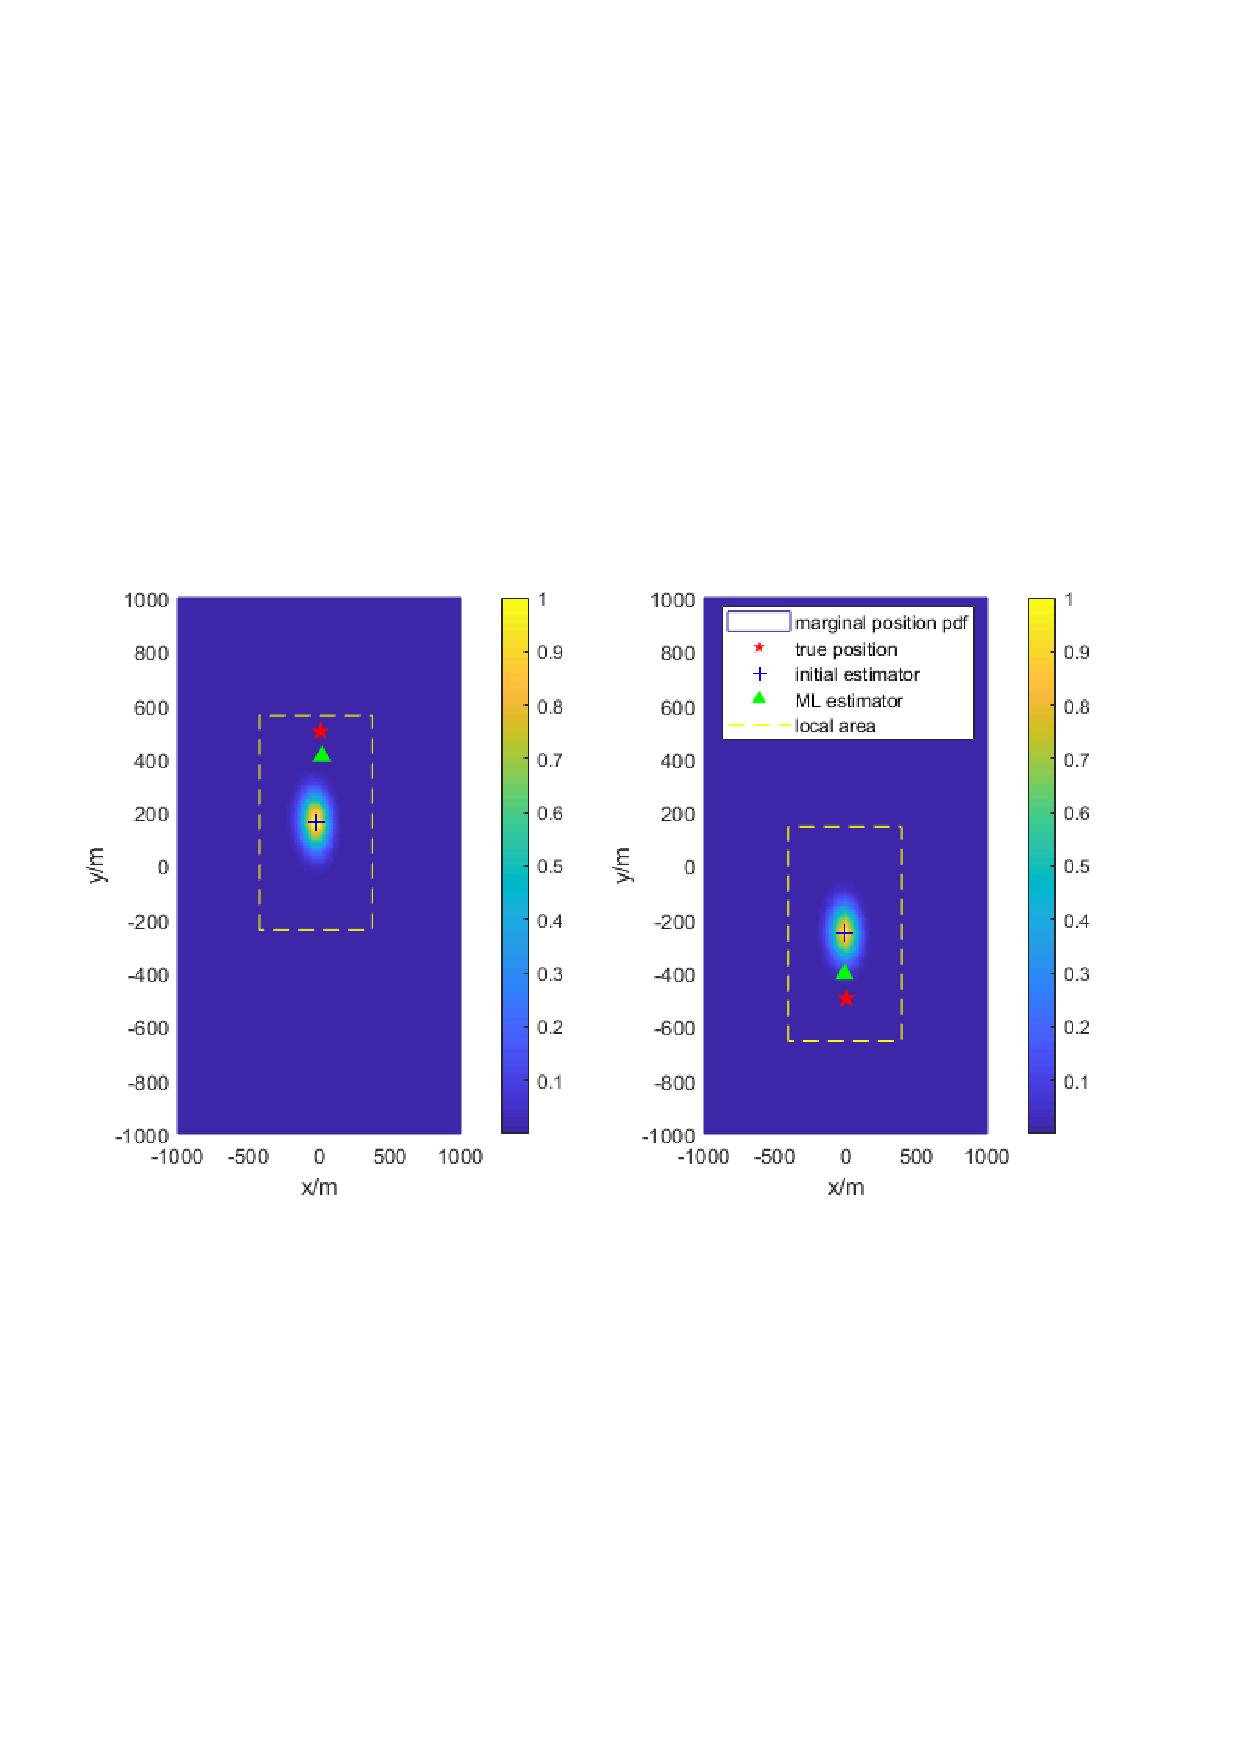
\includegraphics[width=1\textwidth]{pdfFigures/toolarge_rho1=500.pdf}}
    \centering
	\caption{the marginal position pdf, with too large $\rho_1=500$, of two adjacent emitters at $\boldsymbol{p}_1=(0,500)$m and $\boldsymbol{p}_2=(0,-500)$m, the main simulation conditions are Signal to Noise Ratio (SNR)=$15$dB, the number of sections $L=10$, the number of elements $M=3$, the bandwidth $B_w=20kHz$ and the range $\Delta_x=\Delta_y=400$m.}\label{fig1}
\end{figure}

\begin{figure}[!t]
    \centerline{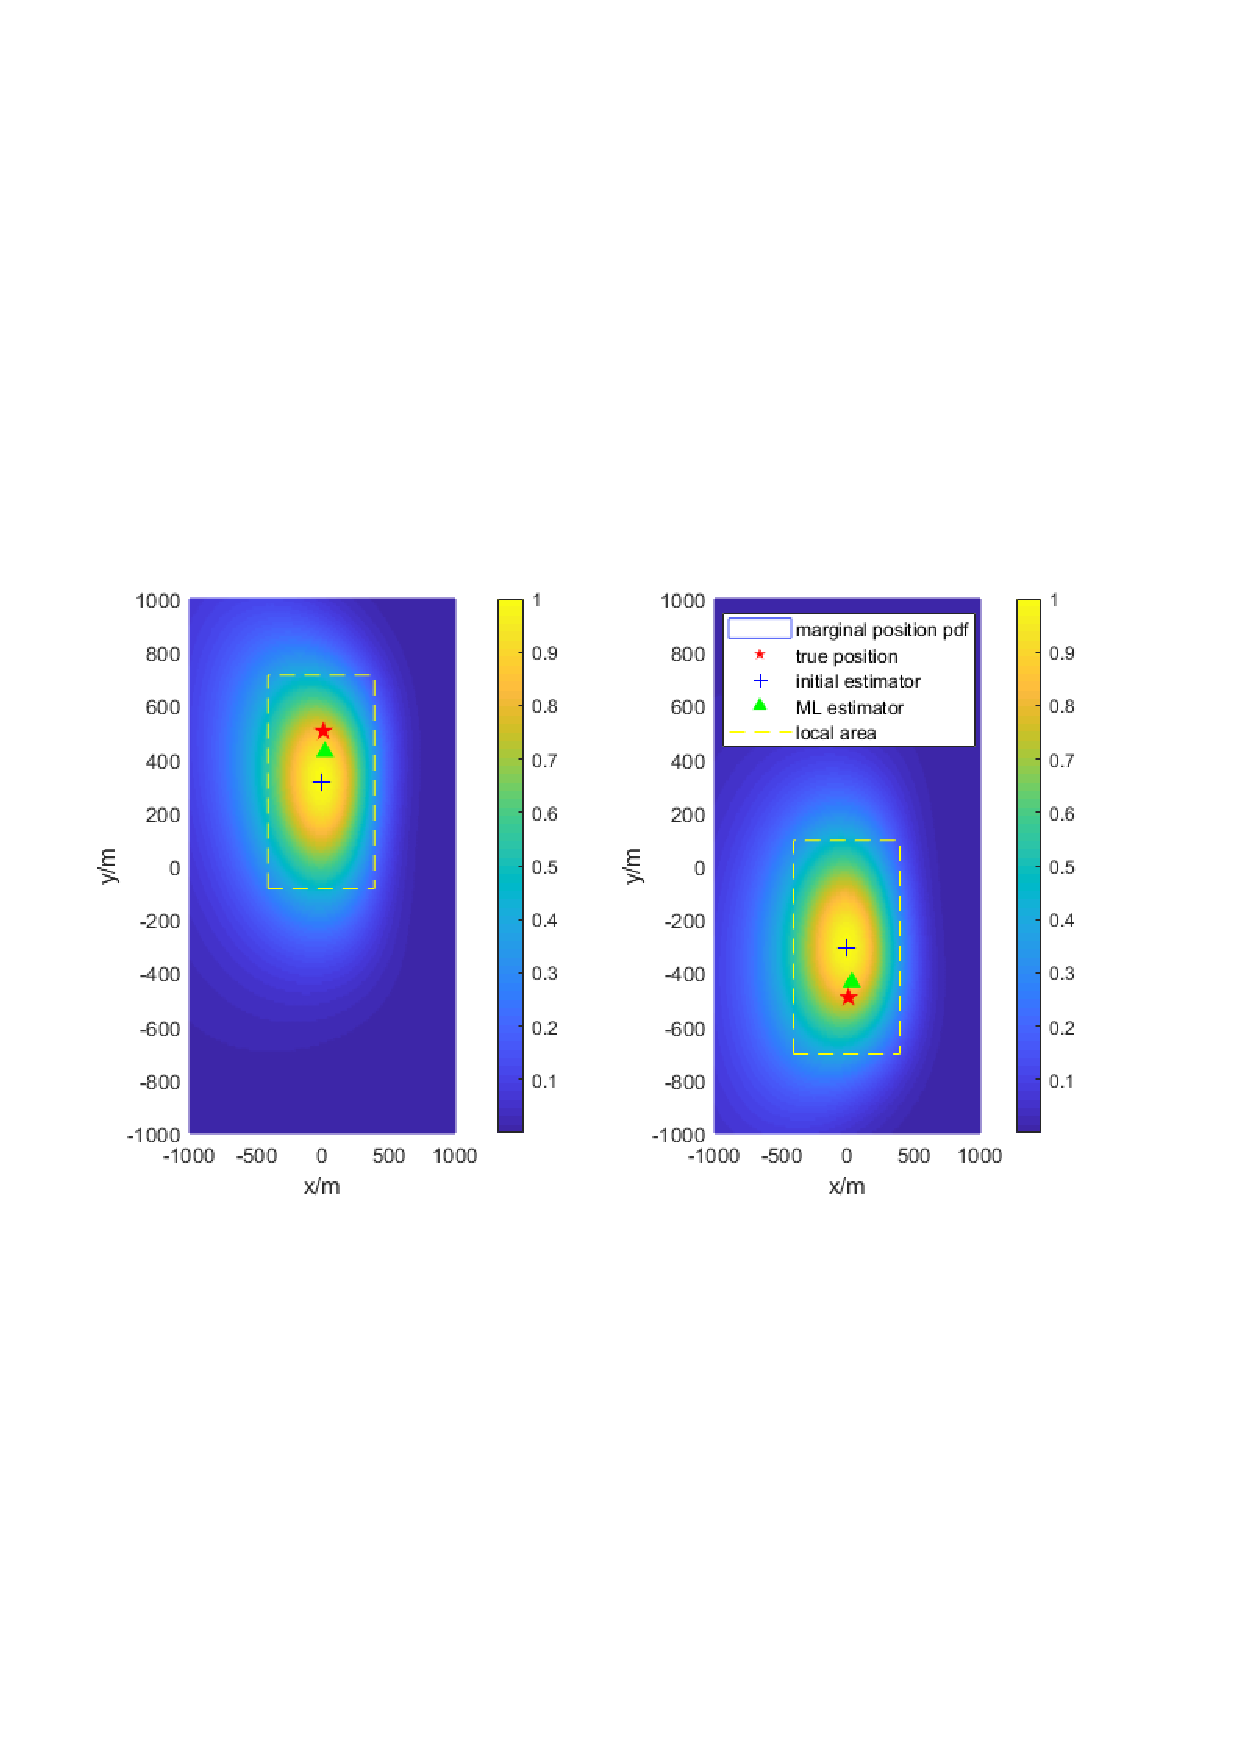
\includegraphics[width=1\textwidth]{pdfFigures/appropriate_rho1=20.pdf}}
    \centering
	\caption{the marginal position pdf with appropriate $\rho_1=20$. Other conditions are the same as the above.}\label{fig2}
\end{figure}

Another detail about the super-parameter $\rho_1$ and $\rho_2$ remained to be stated. The distribution of probability mass in the local area $D_{\mathring{x}_q}\times D_{\mathring{y}_q}$ (or $D_{\mathring{t}_q}$) is governed by the super-parameter $\rho_1$ in the marginal position pdf $g_{q}^{\text{mar}}(x_q,y_q)$ (or $\rho_2$ in the conditional transmitted time pdf $g_{q}^{\text{con}}(\mathring{t}_q\vert \boldsymbol{p}_q^{(r)})$) . Similarly to \eqref{gc}, the probability mass of $g_{q}^{\text{mar}}(x_q,y_q)$ (or $g_{q}^{\text{con}}(\mathring{t}_q\vert \boldsymbol{p}_q^{(r)})$) would concentrate at the location of the maximum peak, $(\mathring{x}_q,\mathring{y}_q)$ (or $\mathring{t}_q$), as $\rho_1$ (or $\rho_2$) increases. The too large $\rho_1$ (or $\rho_2$) would result in that the points, included in local area but far away from the maximum peak point, are hardly to be sampled (as seen in Fig.\ref{fig1}). The range parameter $\Delta_x$, $\Delta_y$ (or $\Delta_{\mathring{t}}$) should, therefore, match with $\rho_1$ (or $\rho_2$), in order to generate the required realizations efficiently (as seen in Fig.\ref{fig2}). 

\section{Numerical Simulation and Discussion}
In this section, we design several numerical simulations to verify and evaluate the performance of the proposed IS based ML estimator, denoted by IS-ML-DPD, and compare it with the decoupled DPD estimator (assuming the number of sections $L\to \infty$) proposed in \cite{DPD2005} and the MVDR based DPD estimator proposed in \cite{Tirer2015High}, denoted by single-ML-DPD and MVDR-DPD respectively. To give an explicit comparison with the ML estimator \eqref{MLE}, we also give its performance curve that are obtained by an iterative local optimization method using the true emitters' positions as the initial point, denoted by optimal-ML-DPD.

\begin{figure}[!t]
    \centerline{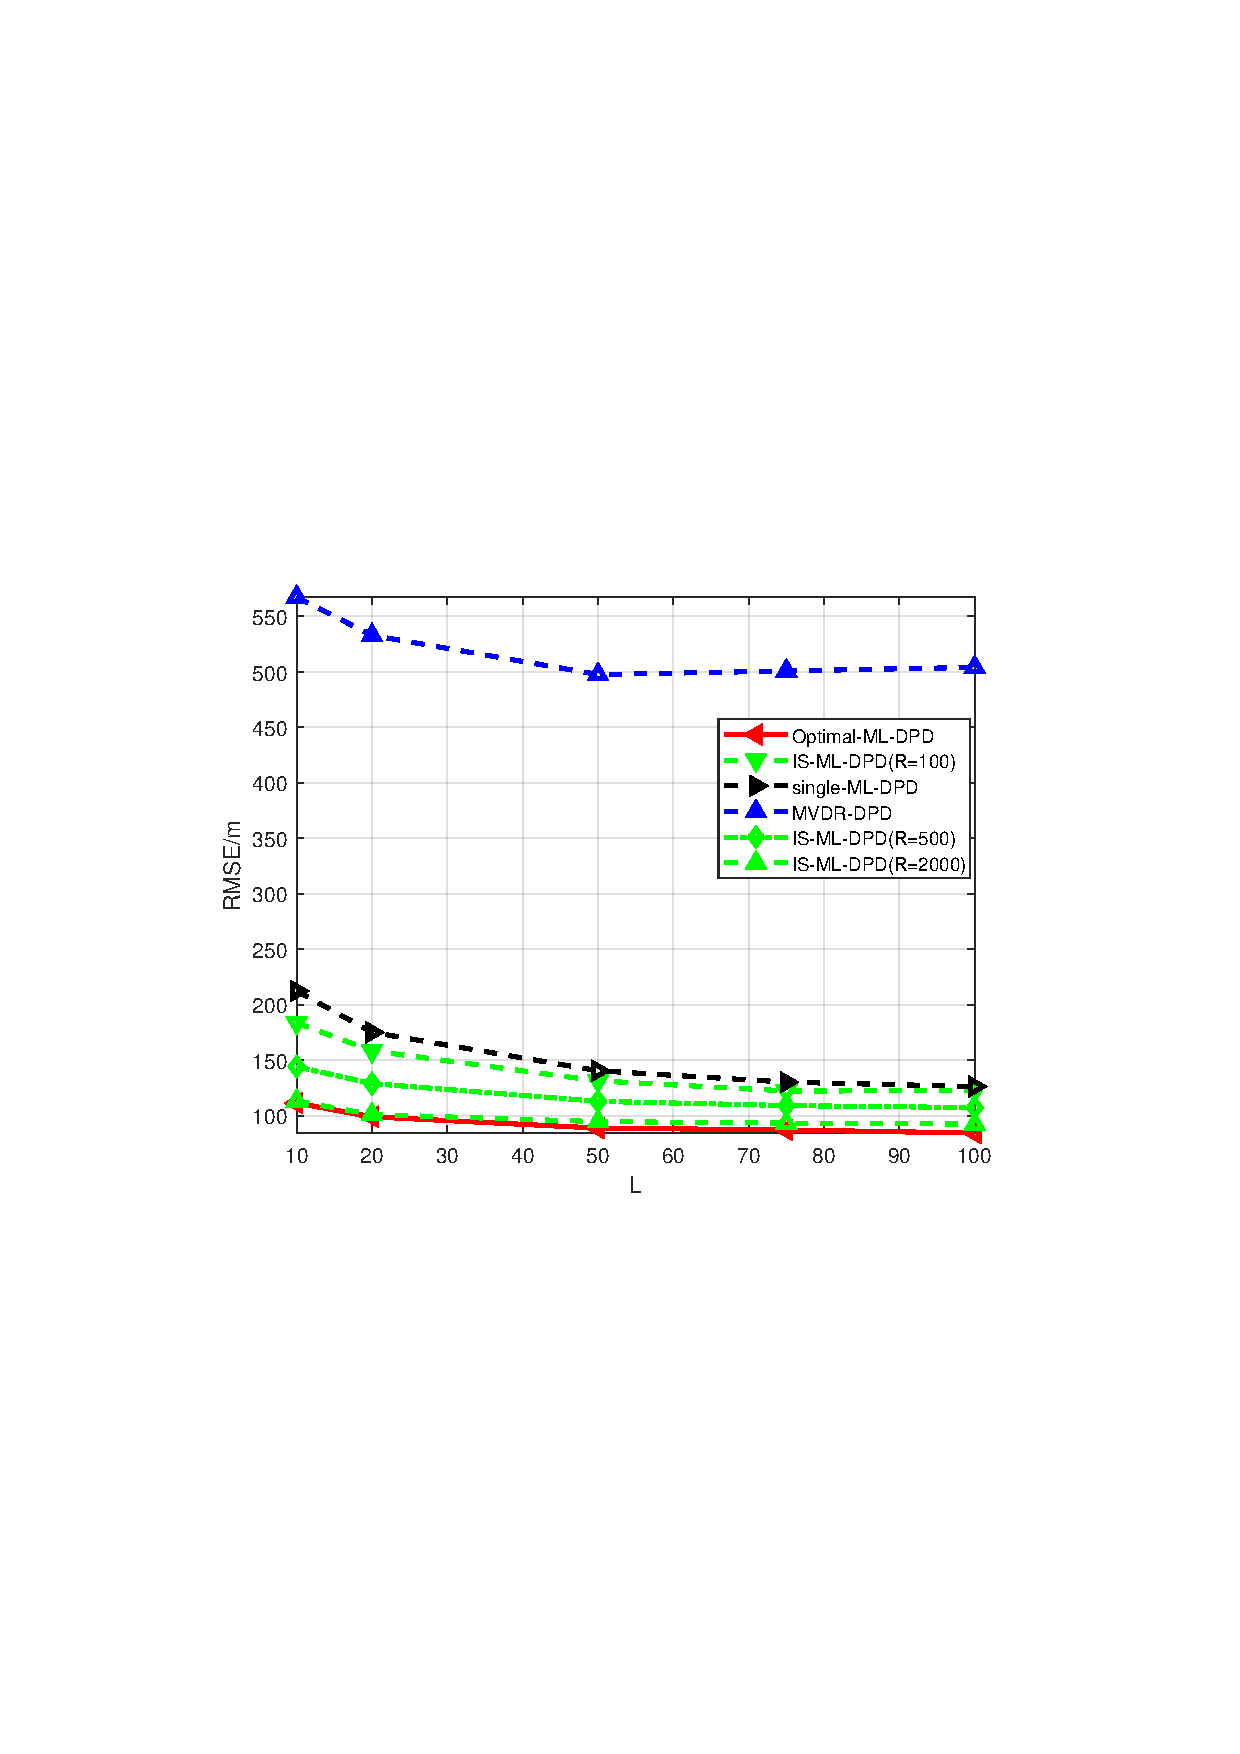
\includegraphics[width=1\textwidth]{pdfFigures/QvsRMSE(opt-IS(R100-500-2000)-SML-MVDR(1))SNR5dB.pdf}}
    \centering
	\caption{the RMSE of each estimator varies with the number of sections $L$.}\label{fig3}
\end{figure}

\begin{figure}[!t]
    \centerline{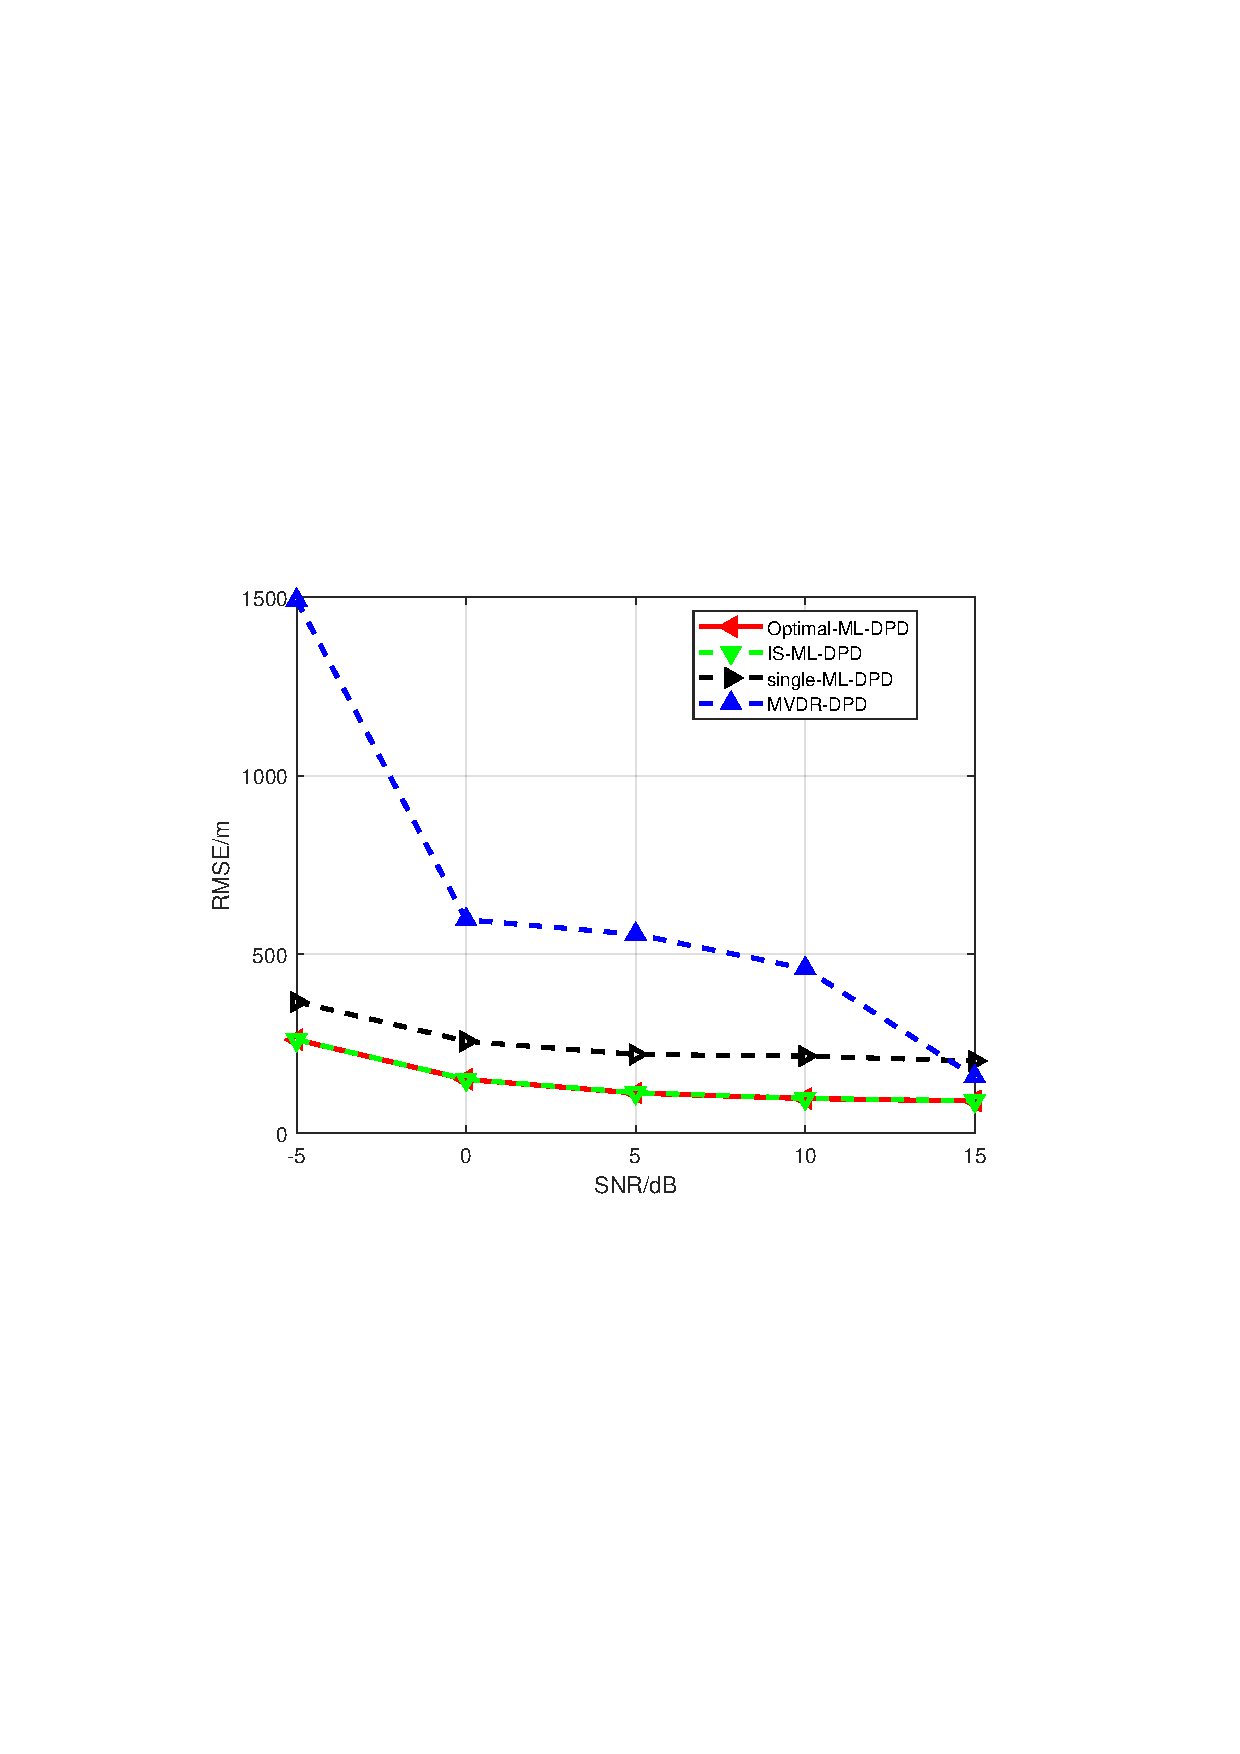
\includegraphics[width=1\textwidth]{pdfFigures/SNRvsRMSE(opt-IS(2000)-SML-MVDR(1))L10.pdf}}
    \centering
	\caption{the RMSE of each estimator varies with the SNR.}\label{fig4}
\end{figure}



\section*{References}
\bibliography{mybibfile}

\end{document}